\documentclass[mathserif]{beamer}              %use this for creating the presentation
%\documentclass[handout,mathserif]{beamer}       %use this for creating the handout (i.e. no animation)
\usepackage{amsmath}
\usepackage{amssymb}
\usepackage{amsthm}
\usepackage{graphicx}
%\usepackage{subfig}

\usecolortheme{orchid}

\newcommand{\alignbox}[1]
    {\begin{equation*} \boxed{ \begin{aligned} #1
    \end{aligned} } \end{equation*}}
\newcommand{\gatherbox}[1]
    {\begin{equation*} \boxed{ \begin{gathered} #1
    \end{gathered} } \end{equation*}}
\newcommand{\drm}{\textrm{d}}
\newcommand{\qmd}{q^{-\drm}}
\newcommand{\paused}{\vspace*{-\baselineskip}\pause}     %use this if \pause puts too much space before the next line

%\input{../commands}
%\setkeys{Gin}{draft=true}

\linespread{1.3}

\title{ME 233 -- Advanced Control II\\
    Lecture 17 \\
    Minimum Variance Regulator}
\author{Tony Kelman}
\institute{UC Berkeley}


\begin{document}

\maketitle

\begin{frame}
    \frametitle{Outline}
    \tableofcontents
\end{frame}

\section{Introduction}
\begin{frame}
    \frametitle{Outline}
    \tableofcontents[currentsection]
\end{frame}

\begin{frame}
    \frametitle{Model Form}

    We consider a state space model of the form
    \begin{align*}
        x(k+1) & = \hat{A} x(k) + \hat{B} u(k) + \hat{B}_w w(k) \\
        y(k) & = \hat{C} x(k) + v(k)
    \end{align*}
    where
    \begin{itemize}
        \item
        $u(k)$ is the \textbf{scalar} control signal

        \item
        $y(k)$ is the \textbf{scalar} measurement signal

        \item
        $w(k)$ is the input noise \\
        (white, zero-mean, $E\{w(k) w^T(k)\} = W$)

        \item
        $v(k)$ is the measurement noise \\
        (white, zero-mean, $E\{v(k) v^T(k)\} = V$)

        \item
        $E\{w(k) v^T(k) \} = 0$

    \end{itemize}
\end{frame}

\begin{frame}
    \frametitle{Stationary Kalman Filter V2 (Review)}

    The optimal state estimator is given by
    \begin{align*}
        \hat{x}^o(k+1) & = \hat{A} \hat{x}^o(k) + \hat{B} u(k) + \hat{L} \tilde{y}^o(k) \\
        \tilde{y}^o(k) & = y(k) - \hat{C} \hat{x}^o(k)
    \end{align*}
    where
    \begin{align*}
        & \hat{L} = \hat{A} M \hat{C}^T [\hat{C} M \hat{C}^T + V]^{-1} \\
        & M = \hat{A} M \hat{A}^T + \hat{B}_w W \hat{B}_w^T
            - \hat{A} M \hat{C}^T [\hat{C} M \hat{C}^T + V]^{-1} \hat{C} M \hat{A}^T \\
        & \hat{A} - \hat{L}\hat{C} \textrm{ is Schur}
    \end{align*}
    \paused

    Also, the signal $\tilde{y}^o(k)$ is zero-mean, white, and has covariance $\hat{C} M \hat{C}^T + V$.

\end{frame}

\begin{frame}
    \frametitle{Alternate Model Form}

    Using the Kalman Filter V2, we can write
    \begin{align*}
        \hat{x}^o(k+1) & = \hat{A} \hat{x}^o(k) + \hat{B} u(k) + \hat{L} \epsilon(k) \\
        y(k) & = \hat{C} \hat{x}^o(k) + \epsilon(k)
    \end{align*}
    where $\epsilon(k) = \tilde{y}^o(k)$.
    \pause

    As a transfer function, this is
    \begin{align*}
        Y(z) & = [\hat{C} (zI - \hat{A})^{-1} \hat{B}] U(z) \\
        & \quad + [1 + \hat{C} (zI - \hat{A})^{-1} \hat{L}] E(z)
    \end{align*}
    \paused

    Recall that $\displaystyle{ 1 + \hat{C} (zI - \hat{A})^{-1} \hat{L} = \frac{\det[zI-(\hat{A}-\hat{L}\hat{C})]}{\det[zI-\hat{A}]} }$

\end{frame}

\begin{frame}
    \frametitle{Alternate Transfer Function Model}

    From the previous slide, we have that
    \begin{align*}
        Y(z) & = \frac{\bar{B}(z)}{\bar{A}(z)} U(z) + \frac{\bar{C}(z)}{\bar{A}(z)} E(z)
    \end{align*}
    \paused

    where
    \begin{align*}
        \bar{A}(z) & = z^n + a_1 z^{n-1} + \cdots + a_n && = \det[zI-\hat{A}] \\
        \bar{C}(z) & = z^n + c_1 z^{n-1} + \cdots + c_n && = \det[zI-(\hat{A}-\hat{L}\hat{C})] \\
        \bar{B}(z) & = b_0 z^m + \cdots + b_m
    \end{align*}
    \paused

    Since $\hat{A}-\hat{L}\hat{C}$ is Schur, the polynomial $\bar{C}(z)$ is Schur

\end{frame}

\begin{frame}
    \frametitle{Polynomials in $q^{-1}$}

    We now define $\drm = n - m$ and the polynomials
    \begin{align*}
        A(z^{-1}) & = z^{-n} \bar{A}(z) && = 1 + a_1 z^{-1} + \cdots + a_n z^{-n} \\
        C(z^{-1}) & = z^{-n} \bar{C}(z) && = 1 + c_1 z^{-1} + \cdots + c_n z^{-n} \\
        B(z^{-1}) & = z^{-m} \bar{B}(z) && = b_0 + b_1 z^{-1} + \cdots + b_m z^{-m} \\
    \end{align*}
    \paused

    so that we can write the transfer function from the previous slide as
    \begin{align*}
        Y(z) & = \frac{z^{-\drm} B(z^{-1})}{A(z^{-1})} U(z) + \frac{C(z^{-1})}{A(z^{-1})} E(z)
    \end{align*}
    \paused

    Note in particular that $C(z^{-1})$ is an anti-Schur polynomial of $z^{-1}$

\end{frame}

\begin{frame}
    \frametitle{ARMAX Plant Model}

    We have now transformed the original state space plant model to
    \begin{align*}
        A(q^{-1}) y(k) = \qmd B(q^{-1}) u(k) + C(q^{-1}) \epsilon(k)
    \end{align*}
    where $C(q^{-1})$ is an anti-Schur polynomial of $q^{-1}$ and $\epsilon(k)$ is zero-mean white noise with covariance $\hat{C} M \hat{C}^T + V$
    \pause

    \vspace{4ex}

    This type of model is called an \underline{ARMAX} model because it is an ARMA model with an eXogenous input.

\end{frame}




\section{MVR Problem Statement}
\begin{frame}
    \frametitle{Outline}
    \tableofcontents[currentsection]
\end{frame}

\begin{frame}
    \frametitle{Minimum Variance Regulator (MVR) Problem}

    Given the ARMAX model
    \begin{align*}
        A(q^{-1}) y(k) = \qmd B(q^{-1}) u(k) + C(q^{-1}) \epsilon(k)
    \end{align*}
    where
    \begin{itemize}
        \item
        $C(q^{-1})$ is an anti-Schur polynomial of $q^{-1}$

        \item
        $B(q^{-1})$ has no zeros on the unit circle

        \item
        $\epsilon(k)$ is zero-mean white noise
        
        \item
        The plant has no unstable pole-zero cancelations, i.e.\ the polynomials $A(q^{-1})$ and $B(q^{-1})$ have no common zeros such that $|q^{-1}| < 1$
    \end{itemize}
    \pause
    
    find the stabilizing feedback control law that minimizes the output variance $E\{y^2(k)\}$
\end{frame}

\section{MVR Solution}
\begin{frame}
    \frametitle{Outline}
    \tableofcontents[currentsection]
\end{frame}

\begin{frame}
    \frametitle{Factorization of $B$ and $\bar{B}$}

    In general, the polynomial $\bar{B}(q) = q^m B(q^{-1})$ has
    \begin{itemize}
        \item
        $m_s$ zeros strictly inside the unit circle (stable plant zeros)

        \item
        $m_u$ zeros strictly outside the unit circle (unstable plant zeros)
    \end{itemize}
    \pause

    Perform the factorization
    \begin{align*}
        B(q^{-1}) = B^s(q^{-1}) B^u(q^{-1})
    \end{align*}
    where
    \begin{itemize}
        \item
        $\bar{B}^s(q) = q^{m_s} B^s(q^{-1})$ has its zeros inside the unit circle \\
        (These are the stable plant zeros)

        \item
        $\bar{B}^u(q) = q^{m_u} B^u(q^{-1})$ has its zeros outside the unit circle \\
        (These are the unstable plant zeros)

        \item
        $\bar{B}^u(0) = 1$
    \end{itemize}

\end{frame}

\begin{frame}
    \frametitle{Minimum Variance Regulator (MVR) Solution}

    \begin{itemize}
        \item
        The optimal control $u_*(k)$ is given by
        \begin{align*}
            B^s(q^{-1}) R(q^{-1}) u_*(k) = - S(q^{-1}) y(k)
        \end{align*}
        where $R(q^{-1})$ and $S(q^{-1})$ are found by solving the Diophantine equation
        \begin{align*}
            C(q^{-1}) \bar{B}^u(q^{-1}) = A(q^{-1}) R(q^{-1}) + \qmd B^u(q^{-1}) S(q^{-1})
        \end{align*}
        where
        \begin{align*}
            R(q^{-1}) & = 1 + r_1 q^{-1} + \cdots + r_{n_r} q^{-n_r} \\
            S(q^{-1}) & = s_0 + s_1 q^{-1} + \cdots + s_{n_s} q^{-n_s}
        \end{align*}
        and $n_r = m_u + \drm - 1$ and $n_s = n-1$

    \end{itemize}
\end{frame}

\begin{frame}
    \frametitle{Minimum Variance Regulator (MVR) Solution}

    \begin{itemize}
        \item
        The optimal cost is 
        \begin{align*}
            E\{y^2(k)\} = E\{\epsilon_f^2(k)\} 
        \end{align*}
        where $\epsilon_f(k)$ is defined in terms of $\epsilon(k)$ by the ARMA model
        \begin{align*}
            \bar{B}^u(q^{-1}) \epsilon_f(k) = R(q^{-1}) \epsilon(k)
        \end{align*}
    \end{itemize}
\end{frame}

\begin{frame}
    \frametitle{Constructing the MVR}

    \begin{enumerate}
        \item
        Find $\hat{L}$ using a stationary Kalman filter design

        \item
        Construct $C(q^{-1}) = q^{-n} \det[qI - (\hat{A} - \hat{L}\hat{C})]$

        \item
        Factor $B(q^{-1}) = B^s(q^{-1}) B^u(q^{-1})$ as described previously \\
        (don't forget that $\bar{B}^u(0) = 1$)

        \item
        Solve the Diophantine equation
        \begin{align*}
            C(q^{-1}) \bar{B}^u(q^{-1}) = A(q^{-1}) R(q^{-1}) + \qmd B^u(q^{-1}) S(q^{-1})
        \end{align*}

        \item
        Form the optimal controller
        \begin{align*}
            B^s(q^{-1}) R(q^{-1}) u_*(k) = - S(q^{-1}) y(k)
        \end{align*}
    \end{enumerate}
\end{frame}

\begin{frame}
    \frametitle{Solution Comments}

    \begin{itemize}
        \item
        Be careful with $B^u(q^{-1})$, $\bar{B}^u(q)$, and $\bar{B}^u(q^{-1})$
        \pause

        \begin{itemize}
            \item
            $B^u(q^{-1})$ is a Schur polynomial in $q^{-1}$
            \pause

            \item
            $\bar{B}^u(q)$ is an anti-Schur polynomial in $q$
            \pause

            \item
            $\bar{B}^u(q^{-1})$ is an anti-Schur polynomial in $q^{-1}$
        \end{itemize}
        \pause

        \item
        Note that the Diophantine equation involves both $B^u(q^{-1})$ and $\bar{B}^u(q^{-1})$.
        \pause

        \item
        Since $\bar{B}^u(q^{-1})$ is anti-Schur, the operator $\displaystyle{\frac{R(q^{-1})}{\bar{B}^u(q^{-1})}}$ is BIBO.
        \paused
        $\displaystyle{\Rightarrow \quad \epsilon_f(k) = \frac{R(q^{-1})}{\bar{B}^u(q^{-1})} \epsilon(k)}$ has bounded covariance

    \end{itemize}
\end{frame}

\begin{frame}
    \frametitle{Special Case: $B(q^{-1})$ is anti-Schur}

    When $B(q^{-1})$ is anti-Schur, we have
    \begin{itemize}
        \item
        $B^s(q^{-1}) = B(q^{-1})$

        \item
        $B^u(q^{-1}) = \bar{B}^u(q) = \bar{B}^u(q^{-1}) = 1$
        \pause

        \item
        Expressing $R(q^{-1}) = 1 + r_1 q^{-1} + \cdots + r_{n_r} q^{-n_r}$, the optimal cost is
        \begin{align*}
            E\{y^2(k)\}
            & = E\{[R(q^{-1})\epsilon(k)]^2\} \\
            & = E\{[\epsilon(k) + r_1 \epsilon(k-1) + \cdots + r_{n_r} \epsilon(k-n_r)]^2 \} \\
            & = E\{\epsilon^2(k)\} + r_1^2 E\{\epsilon^2(k-1)\} + \cdots + r_{n_r}^2 E\{\epsilon^2(k-n_r)\} \\
            & = (1 + r_1^2 + \cdots + r_{n_r}^2) E\{\epsilon^2(k)\}
        \end{align*}
        \pause
        Therefore
        \alignbox{
            E\{y^2(k)\} = (1 + r_1^2 + \cdots + r_{n_r}^2) (\hat{C}M\hat{C}^T + V)
        }

    \end{itemize}
\end{frame}

\section{Proof, Special Case: $B(q^{-1})$ Anti-Schur}
\begin{frame}
    \frametitle{Outline}
    \tableofcontents[currentsection]
\end{frame}

\begin{frame}
    \frametitle{Proof Methodology}

    The proof will be done in 4 parts:

    \begin{enumerate}
        \item
        Rewrite the system dynamics in a more convenient form
        \pause

        \item
        Prove that $E\{z(k-\drm) \epsilon_f(k)\} = 0$, where $z(k)$ is a sequence to be defined in subsequent slides
        \pause

        \item
        Prove optimality of proposed control scheme
        \pause

        \item
        Verify closed-loop stability

    \end{enumerate}
    \pause

    Comments on the notation in this proof:
    \begin{itemize}
        \item
        Capital letters always denote polynomials; lower case letters denote sequences (except $\drm$ and $q$)

        \item
        Dependency of polynomials on $q^{-1}$ will be omitted\\
        e.g. $\bar{B}^u$ will refer to $\bar{B}^u(q^{-1})$

        \item
        Dependency of sequences on $k$ will be omitted\\
        e.g. $y$ will refer to $y(k)$

    \end{itemize}
\end{frame}

\begin{frame}
    \frametitle{Part 1: Rewrite Dynamics}

    The plant dynamics are
    \begin{align*}
        Ay = \qmd Bu + C \epsilon
    \end{align*}
    and the Diophantine equation gives
    \begin{align*}
        [RA]y = [C - \qmd S] y
    \end{align*}
    \paused

    Combining these two equations gives
    \begin{align*}
        R [\qmd Bu + C \epsilon] = [C - \qmd S] y
    \end{align*}
    \paused
    \begin{align*}
        \Rightarrow \quad Cy - \qmd(Sy + BRu) - CR\epsilon = 0
    \end{align*}

\end{frame}

\begin{frame}
    \frametitle{Part 1: Rewrite Dynamics}

    From the previous slide:
    \begin{align*}
        \quad Cy - \qmd(Sy + BRu) - CR\epsilon = 0
    \end{align*}

    \begin{itemize}
        \item
        Define $z(k)$ in terms of $y(k)$ and $u(k)$ using
        \begin{align*}
            Cz = Sy + BRu
        \end{align*}
        (note that we are not necessarily using the optimal control)
        \pause

        \item
        Define $\epsilon_f = R\epsilon$
        \pause

        \item
        From the top equation,
        \begin{gather*}
            Cy - \qmd Cz - C\epsilon_f = 0 \qquad \Rightarrow \qquad C (y - \qmd z - \epsilon_f) = 0
        \end{gather*}
        \pause
        Since $C$ is anti-Schur, we have $y - \qmd z - \epsilon_f \longrightarrow 0$
        \pause

        \alignbox{
            y(k) = z(k-\drm) + \epsilon_f(k)
        }
    \end{itemize}
\end{frame}

\begin{frame}
    \frametitle{Part 2: $E\{z(k-\drm)\epsilon_f(k)\} = 0$}

    \begin{itemize}
        \item
        Since $\epsilon(k) = y(k) - E\{y(k) | y(k-1),y(k-2),\ldots\}$, we use least squares property 1 to see that
        \begin{align*}
            E \{ y(k-\ell) \epsilon(k+p) \}, \qquad \forall \ell > 0, p \geq 0
        \end{align*}
        \paused

        \item
        $\epsilon_f(k+\drm-1) = \epsilon(k+\drm-1) + r_1 \epsilon(k+\drm-2) + \cdots + r_{\drm-1} \epsilon(k)$
        \begin{align*}
            \Rightarrow \quad E \{ y(k-\ell) \epsilon_f(k+\drm-1) \} = 0 \qquad \forall \ell > 0
        \end{align*}
        \paused

        \item
        Since $u(k)$ is a function of $y(k),y(k-1),\ldots$
        \begin{align*}
            E \{ u(k-\ell) \epsilon_f(k+\drm-1) \} = 0 \qquad \forall \ell > 0
        \end{align*}
        \paused

        \item
        Since $z(k)$ is a function of $y(k),y(k-1),\ldots$ and $u(k),u(k-1),\ldots$
        \begin{align*}
            E \{ z(k-\ell) \epsilon_f(k+\drm-1) \} = 0 \qquad \forall \ell > 0
        \end{align*}
        \paused

        \item
        Choosing $\ell = 1$ completes part 2
    \end{itemize}
\end{frame}

\begin{frame}
    \frametitle{Part 3: Optimal Control}

    Recall that
    \begin{gather*}
        y(k) = z(k-\drm) + \epsilon_f(k) \\
        E\{z(k-\drm)\epsilon_f(k)\} = 0
    \end{gather*}
    \paused
    Therefore,
    \begin{align*}
        E\{y^2(k)\} = E\{z^2(k-\drm)\} + E\{\epsilon_f^2(k)\}
    \end{align*}
    \paused

    Notes:
    \begin{itemize}
        \item
        At this point, we have only assumed that $u(k)$ stabilizes the system (so that the relevant covariances are bounded)
        \pause

        \item
        $E\{\epsilon_f^2(k)\}$ does not depend on the choice of the control law
        \pause

        \item
        $\Rightarrow$ We would like to choose $u$ to minimize $E\{z^2\}$
        \pause

        \item
        If we can make $E\{z^2\} = 0$, the control must be optimal
    \end{itemize}

\end{frame}

\begin{frame}
    \frametitle{Part 3: Optimal Control}

    Goal: choose $u$ so that $E\{z^2\} = 0$
    \pause

    \begin{itemize}
        \item
        If we apply the control signal $u_*(k)$ defined by
        \begin{align*}
            BRu_* = - Sy
        \end{align*}
        \paused
        we have
        \begin{align*}
            Cz = BRu_* + Sy = 0
        \end{align*}
        \paused

        \item
        $C(q^{-1})$ is an anti-Schur polynomial $\Rightarrow \ z(k) \longrightarrow 0$.
        \pause

        \item
        For this control signal, $E\{z^2\} = 0$, which means that $u_*(k)$ is optimal, provided that the closed-loop system is stable
        \pause

        \item
        Also note that $E\{y^2\} = E\{\epsilon_f^2\}$, provided that the closed-loop system is stable
    \end{itemize}
\end{frame}

\begin{frame}
    \frametitle{Part 4: Closed-loop stability}

    From the plant dynamics and feedback law, we have
    \begin{align*}
        \begin{bmatrix}
                A & -\qmd B \\
                S & BR
            \end{bmatrix} \begin{bmatrix}
                y \\
                u
            \end{bmatrix} = \begin{bmatrix}
                C\epsilon \\
                0
            \end{bmatrix}
    \end{align*}
    \pause
    \begin{align*}
        \Rightarrow \begin{bmatrix}
                y \\
                u
            \end{bmatrix} & = \frac{1}{BAR + \qmd BS} \begin{bmatrix}
                BR & \qmd B \\
                -S & A
            \end{bmatrix} \begin{bmatrix}
                C\epsilon \\
                0
            \end{bmatrix} \\
        & = \frac{1}{B(AR + \qmd S)} \begin{bmatrix}
                BRC\epsilon \\
                -SC\epsilon
            \end{bmatrix} = \frac{1}{BC} \begin{bmatrix}
                BRC\epsilon \\
                -SC\epsilon
            \end{bmatrix}
    \end{align*}
    \paused

    Since $C(q^{-1}) B(q^{-1})$ is an anti-Schur polynomial of $q^{-1}$, the closed-loop system is stable
    \hfill $\blacksquare$

\end{frame}


\section{A-causal but BIBO Systems}
\begin{frame}
    \frametitle{Outline}
    \tableofcontents[currentsection]
\end{frame}

\begin{frame}
    \frametitle{A-causal but BIBO Systems}

    Recall that the polynomial $B^u(q^{-1})$ is Schur
    \pause

    $\,$

    The AR model $B^u(q^{-1}) y(k) = u(k)$ corresponds to the block diagram
    \begin{figure}
        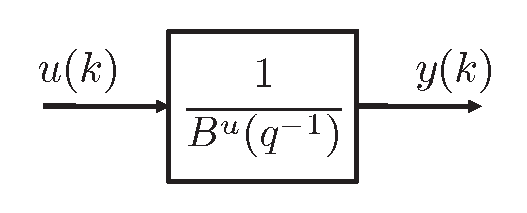
\includegraphics[width=4cm]{MVR_figs_ac1}
    \end{figure}
    \pause


    We can interpret the operator $\displaystyle{ \frac{1}{B^u(q^{-1})} }$ in two ways:
    \pause
    \begin{enumerate}
        \item
        Causal, but unstable
        \pause

        \item
        A-causal, but BIBO
    \end{enumerate}
\end{frame}

\begin{frame}
    \frametitle{Interpretation 1: Causal, but Unstable}

    We are considering the AR model $B^u(q^{-1}) y(k) = u(k)$ where
    \begin{align*}
        B^u(q^{-1}) = 1 + b_1^u q^{-1} + \cdots + b_{m_u}^u q^{-m_u}
    \end{align*}
    \paused
    \begin{align*}
        \longrightarrow \qquad (1 + b_1^u q^{-1} + \cdots + b_{m_u}^u q^{-m_u}) y(k) = u(k)
    \end{align*}
    \pause

    Interpreting the AR model as causal, but unstable corresponds to
    \begin{align*}
        y(k) & = u(k) - [b_1^u q^{-1} + \cdots + b_{m_u}^u q^{-m_u}] y(k) \\
        & = u(k) - b_1^u \, y(k-1) - \cdots - b_{m_u}^u \, y(k-m_u)
    \end{align*}
    \paused

    $\longrightarrow \qquad y(k)$ is a function of $u(k),u(k-1),u(k-2),\ldots$
\end{frame}

\begin{frame}
    \frametitle{Interpretation 2: A-causal, but BIBO}

    We are considering the AR model
    \begin{align*}
        (1 + b_1^u q^{-1} + \cdots + b_{m_u}^u q^{-m_u}) y(k) = u(k)
    \end{align*}
    \paused

    Interpreting the AR model as a-causal, but BIBO corresponds to
    \begin{align*}
        b_{m_u}^u q^{-m_u} y(k) & = u(k) - [1 + b_1^u q^{-1} + \cdots + b_{m_u-1}^u q^{-m_u+1}] y(k)
    \end{align*}
    \paused
    \begin{align*}
        \Rightarrow b_{m_u}^u y(k) & = q^{m_u} u(k) - [q^{m_u} + b_1^u q^{m_u-1} + \cdots + b_{m_u-1}^u q] y(k) \\
        \Rightarrow y(k) & = \frac{1}{b_{m_u}} [ u(k+m_u) - y(k+m_u) - b_1^u y(k+m_u-1) \\
        & \quad - \cdots - b_{m_u-1}^u y(k+1) ]
    \end{align*}
    \paused

    \alignbox{
        y(k) \textrm{ is a function of } u(k+m_u),u(k+m_u+1),u(k+m_u+2),\ldots
    }
\end{frame}

\begin{frame}
    \frametitle{A-causal but BIBO All-Pass Filter}

    Let $w(k)$ be the output of the a-causal, but BIBO ARMAX model
    \begin{align*}
        B^u(q^{-1}) w(k) = \bar{B}^u(q^{-1}) y(k)
    \end{align*}
    This corresponds to the block diagram
    \begin{figure}
        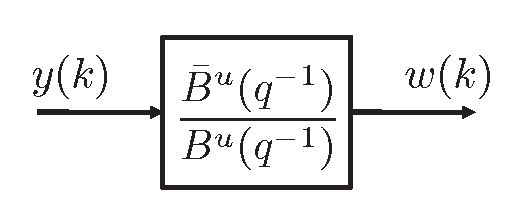
\includegraphics[width=4cm]{MVR_figs_ac2}
    \end{figure}
    \pause

    \textbf{Claim:}
    \begin{align*}
        \left| \frac{\bar{B}^u(e^{-j\omega})}{B^u(e^{-j\omega})} \right| = 1 \qquad \forall \omega \in [0,2\pi]
    \end{align*}
    \paused

    \textit{Proof:}
    \begin{gather*}
        \bar{B}^u(q) = q^{m_u} B^u(q^{-1}) \quad \Rightarrow \quad \bar{B}^u(q^{-1}) = q^{-m_u} B^u(q) \\
        \Rightarrow \quad | \bar{B}^u(e^{-j\omega}) | = | e^{-j\omega m_u} B^u(e^{j\omega}) | = | B^u(e^{j\omega}) |
            = | B^u(e^{-j\omega}) | \qquad \blacksquare
    \end{gather*}

\end{frame}

\begin{frame}
    \frametitle{A-causal but BIBO All-Pass Filter}

    \begin{figure}
        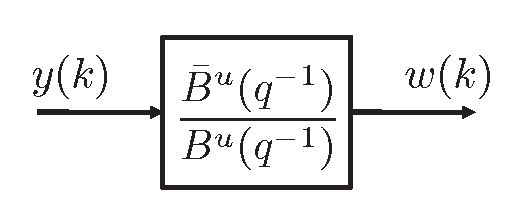
\includegraphics[width=4cm]{MVR_figs_ac2}
    \end{figure}

    The power spectral density of $w(k)$ is
    \begin{align*}
        \Phi_{WW}(\omega) = \left| \frac{\bar{B}^u(e^{-j\omega})}{B^u(e^{-j\omega})} \right|^2 \Phi_{YY}(\omega)
            = \Phi_{YY}(\omega)
    \end{align*}
    \pause

    Therefore
    \begin{align*}
        \Lambda_{WW}(0) = \frac{1}{2\pi} \int_{-\pi}^\pi \Phi_{WW}(\omega) d\omega
            = \frac{1}{2\pi} \int_{-\pi}^\pi \Phi_{YY}(\omega) d\omega
            = \Lambda_{YY}(0)
    \end{align*}
    \pause

    \alignbox{
        E\{w^2(k)\} = E\{y^2(k)\}
    }

\end{frame} 
\section{Proof, General Case}
\begin{frame}
    \frametitle{Outline}
    \tableofcontents[currentsection]
\end{frame}

\begin{frame}
    \frametitle{Proof Methodology}

    The proof will be done in 4 parts:

    \begin{enumerate}
        \item
        Rewrite the system dynamics in a more convenient form
        \pause

        \item
        Prove that $E\{z(k-\drm) \epsilon_f(k)\} = 0$, where $z(k)$ is a sequence to be defined in subsequent slides
        \pause

        \item
        Prove optimality of proposed control scheme
        \pause

        \item
        Verify closed-loop stability

    \end{enumerate}
    \pause

    Comments on the notation in this proof:
    \begin{itemize}
        \item
        Capital letters always denote polynomials; lower case letters denote sequences (except $\drm$ and $q$)

        \item
        Dependency of polynomials on $q^{-1}$ will be omitted\\
        e.g. $\bar{B}^u$ will refer to $\bar{B}^u(q^{-1})$

        \item
        Dependency of sequences on $k$ will be omitted\\
        e.g. $y$ will refer to $y(k)$

    \end{itemize}
\end{frame}

\begin{frame}
    \frametitle{Part 1: Rewrite Dynamics}

    The plant dynamics are
    \begin{align*}
        Ay = \qmd Bu + C \epsilon
    \end{align*}
    and the Diophantine equation gives
    \begin{align*}
        [RA]y = [C\bar{B}^u - \qmd B^u S] y
    \end{align*}
    \paused

    Combining these two equations gives
    \begin{align*}
        R [\qmd Bu + C \epsilon] = [C\bar{B}^u - \qmd B^u S] y
    \end{align*}
    \paused
    \begin{align*}
        \Rightarrow \quad C\bar{B}^u y - \qmd(B^u Sy + BRu) - CR\epsilon = 0
    \end{align*}
    \paused

    Factoring $B^u$ out of the term in parentheses yields
    \begin{align*}
        \Rightarrow \quad C\bar{B}^u y - \qmd B^u (Sy + B^s Ru) - CR\epsilon = 0
    \end{align*}
\end{frame}

\begin{frame}
    \frametitle{Part 1: Rewrite Dynamics}

    From the previous slide:
    \begin{align*}
        C\bar{B}^u y - \qmd B^u (Sy + B^s Ru) - CR\epsilon = 0
    \end{align*}

    \begin{itemize}
        \item
        Define $z(k)$ in terms of $y(k)$ and $u(k)$ using
        \begin{align*}
            Cz = Sy + B^s Ru
        \end{align*}
        (note that we are not necessarily using the optimal control)
        \pause

        \item
        Define $\bar{\epsilon}_f$ and $w$ by
        \begin{align*}
            B^u \bar{\epsilon}_f & = R\epsilon
                & B^u w = \bar{B}^u y
        \end{align*}
        We interpret these relationships as a-causal, but BIBO
        \pause

        \item
        From the top equation,
        \begin{gather*}
            CB^u w - \qmd CB^u z - CB^u \bar{\epsilon}_f = 0 \\
            \Rightarrow CB^u (w - \qmd z - \bar{\epsilon}_f) = 0
        \end{gather*}
    \end{itemize}
\end{frame}

\begin{frame}
    \frametitle{Part 1: Rewrite Dynamics}

    So far, we know that
    \begin{align*}
        CB^u (w - \qmd z - \bar{\epsilon}_f) = 0
    \end{align*}

    \begin{itemize}
        \item
        Since $C$ is anti-Schur, we have $B^u (w - \qmd z - \bar{\epsilon}_f) \longrightarrow 0$
        \pause

        \item
        If we regard $\displaystyle{\frac{1}{B^u(q^{-1})}}$ as a-causal but BIBO, we have $w - \qmd z - \bar{\epsilon}_f \longrightarrow 0$
        \pause

        \item
        We have now obtained
        \alignbox{
            w(k) = z(k-\drm) + \bar{\epsilon}_f(k)
        }
        \paused

        \item
        Also note that, because $\displaystyle{w(k) = \frac{\bar{B}^u(q^{-1})}{B^u(q^{-1})} y(k)}$
        \alignbox{
            E\{w^2(k)\} = E\{y^2(k)\}
        }
    \end{itemize}

\end{frame}

\begin{frame}
    \frametitle{Part 2: $E\{z(k-\drm)\bar{\epsilon}_f(k)\} = 0$}

    \begin{itemize}
        \item
        Since $\epsilon(k) = y(k) - E\{y(k) | y(k-1),y(k-2),\ldots\}$, we use least squares property 1 to see that
        \begin{align*}
            E \{ y(k-\ell) \epsilon(k+p) \}, \qquad \forall \ell > 0, p \geq 0
        \end{align*}
        \paused

        \item
        Defining $\epsilon_r = R\epsilon$, we have
        \begin{gather*}
            \epsilon_r(k+n_r) = \epsilon(k+n_r) + r_1 \epsilon(k+n_r-1)
                + \cdots + r_{n_r} \epsilon(k) \\
            \Rightarrow \quad E \{ y(k-\ell) \epsilon_r(k + n_r + p) \} = 0
                \qquad \forall \ell > 0, p \geq 0
        \end{gather*}
        \paused

        \item
        Regarding the relationship $B^u \bar{\epsilon}_f = \epsilon_r$ as a-causal but BIBO, and noting that $n_r = m_u+\drm-1$, we see that $\bar{\epsilon}_f(k+\drm-1)$ is a function of $\epsilon_r(k+n_r)$, $\epsilon_r(k+n_r+1),\cdots$, which implies
        \pause
        \begin{align*}
            E \{ y(k-\ell) \bar{\epsilon}_f(k+\drm-1) \} = 0 \qquad \forall \ell > 0
        \end{align*}
    \end{itemize}
\end{frame}

\begin{frame}
    \frametitle{Part 2: $E\{z(k-\drm)\bar{\epsilon}_f(k)\} = 0$}

    \begin{itemize}
        \item
        Since $u(k)$ is a function of $y(k),y(k-1),\ldots$
        \begin{align*}
            E \{ u(k-\ell) \bar{\epsilon}_f(k+\drm-1) \} = 0 \qquad \forall \ell > 0
        \end{align*}
        \paused

        \item
        Since $z(k)$ is a function of $y(k),y(k-1),\ldots$ and $u(k),u(k-1),\ldots$
        \begin{align*}
            E \{ z(k-\ell) \bar{\epsilon}_f(k+\drm-1) \} = 0 \qquad \forall \ell > 0
        \end{align*}
        \paused

        \item
        Choosing $\ell = 1$ yields
        \begin{align*}
            E\{z(k-\drm)\bar{\epsilon}_f(k)\} = 0
        \end{align*}
    \end{itemize}
\end{frame}

\begin{frame}
    \frametitle{Part 3: Optimal Control}

    So far, we know
    \vspace{-\baselineskip}
    \begin{gather*}
        w(k) = z(k-\drm) + \bar{\epsilon}_f(k) \\
        E\{z(k-\drm)\bar{\epsilon}_f(k)\} = 0 \\
        E\{y^2(k)\} = E\{w^2(k)\}
    \end{gather*}
    \paused
    \begin{align*}
        \Rightarrow E\{y^2(k)\} = E\{z^2(k-\drm)\} + E\{\bar{\epsilon}_f^2(k)\}
    \end{align*}
    \paused

    Notes:
    \begin{itemize}
        \item
        At this point, we have only assumed that $u(k)$ stabilizes the system (so that the relevant covariances are bounded)
        \pause

        \item
        The value of $E\{\bar{\epsilon}_f^2(k)\}$ does not depend on the control law
        \pause

        \item
        $\Rightarrow$ We would like to choose $u$ to minimize $E\{z^2\}$
        \pause

        \item
        If we can make $E\{z^2\} = 0$, the control must be optimal
    \end{itemize}

\end{frame}

\begin{frame}
    \frametitle{Part 3: Optimal Control}

    Goal: choose $u$ so that $E\{z^2\} = 0$
    \pause

    \begin{itemize}
        \item
        If we apply the control signal $u_*(k)$ defined by
        \begin{align*}
            B^s Ru_* = - Sy
        \end{align*}
        \paused
        we have
        \begin{align*}
            Cz = B^s Ru_* + Sy = 0
        \end{align*}
        \paused

        \item
        $C(q^{-1})$ is an anti-Schur polynomial $\Rightarrow \ z(k) \longrightarrow 0$.
        \pause

        \item
        For this control signal, $E\{z^2\} = 0$, which means that $u_*(k)$ is optimal, provided that the closed-loop system is stable.
        \pause

        \item
        Also note that $E\{y^2\} = E\{\bar{\epsilon}_f^2\}$, provided that the closed-loop system is stable
    \end{itemize}
\end{frame}

\begin{frame}
    \frametitle{Part 3: Optimal Control}

    \begin{itemize}
        \item
        Provided that the closed-loop system is stable, we have $E \{ y^2 \} = E \{ \bar{\epsilon}_f^2 \}$ where $\bar{\epsilon}_f$ is generated by the BIBO a-causal ARMA model $B^u \bar{\epsilon}_f = R \epsilon$
        \pause

        \item
        We can instead express the optimal cost in terms of a BIBO causal ARMA model as
        \alignbox{
            E \{ y^2 \} = E \{ \epsilon_f^2 \} \textrm{ where $\epsilon_f$ is the output of } \bar{B}^u \epsilon_f = R \epsilon
        }
        \paused
        \\
        (Remember that $\bar{B}^u$ refers to $\bar{B}^u(q^{-1})$)

        \item
        To see this, note that since $\bar{\epsilon}_f$ is the output of the a-causal but BIBO ARMA model $B^u \bar{\epsilon}_f = \bar{B}^u \epsilon_f$ and the operator $\displaystyle{ \left(\frac{\bar{B}^u}{B^u}\right) }$ is an a-causal all-pass filter, we have that $E\{\epsilon_f^2 \} = E\{\bar{\epsilon}_f^2\}$

    \end{itemize}

\end{frame}

\begin{frame}
    \frametitle{Part 4: Closed-loop stability}

    From the plant dynamics and feedback law, we have
    \begin{align*}
        \begin{bmatrix}
                A & -\qmd B \\
                S & B^s R
            \end{bmatrix} \begin{bmatrix}
                y \\
                u
            \end{bmatrix} = \begin{bmatrix}
                C\epsilon \\
                0
            \end{bmatrix}
    \end{align*}
    \pause
    \begin{align*}
        \Rightarrow \begin{bmatrix}
                y \\
                u
            \end{bmatrix} & = \frac{1}{B^s AR + \qmd BS} \begin{bmatrix}
                B^s R & \qmd B \\
                -S & A
            \end{bmatrix} \begin{bmatrix}
                C\epsilon \\
                0
            \end{bmatrix} \\
        & = \frac{1}{B^s (AR + \qmd B^uS)} \begin{bmatrix}
                B^s RC\epsilon \\
                -SC\epsilon
            \end{bmatrix} = \frac{1}{C \bar{B}^u B^s} \begin{bmatrix}
                B^s RC\epsilon \\
                -SC\epsilon
            \end{bmatrix}
    \end{align*}
    \pause

    Since $C(q^{-1}) \bar{B}^u(q^{-1}) B^s(q^{-1})$ is an anti-Schur polynomial of $q^{-1}$, the closed-loop system is stable
    \hfill $\blacksquare$

\end{frame}



\end{document} 
